\chapter{Results} \label{chapter:5}
The three core metrics which will be compared are coverage availability (as a percentage of time), capacity throughput (Mbps) and latency (ms). 

Coverage availability determines how often the user has service, this metric is based on visibility of satellites and a high level model of the beam-width of a given satellite. This will be compared to urban and rural 5G networks. Throughput is measured in Mbps, this is averaged over a period of time and will also be compared to urban and rural 5G throughput. 

Due to computational limitations of the system on which the simulations were executed, the initial simulation windows analyzed are limited to 12-hour periods. Specifically, simulations were conducted from 08:00 to 20:00 on Thursday, 23 April 2026. All reported results represent averages over this time interval.
All TLE data used in these simulations were obtained and stored on the morning of 23 April 2026. Each simulation was subsequently run using this same TLE dataset and over the same UTC time window, regardless of the actual execution date of the simulation. The selection of this date was arbitrary.

\section{5G performance metrics}
It is important to have a baseline for performance, all future results will be compared to 5G network performance metrics. 

\section{Population Density of Ireland}
To help understand if LEO constellations as they stand can help deliver rural connectivity and or relieve some load from existing networks in more urban areas, it is import to know what areas have what population. 

\section{Starlink Simulation - 08:00 to 20:00, 23 April 2026}
Of the three systems modelled, Starlink has the strongest coverage available in Ireland. This result is somewhat predictable as there are significantly more satellites in Starlink's constellation with the data set used in this project containing 10,188 satellites for Starlink alone. 

In Figure \ref{fig:StarlinkCoverage-percentage}, the average coverage time as a percentage can be seen. The max coverage in Ireland was found to be $75.38\%$ time over the 12 hour period modelled here. The coverage is strongly skewed towards the midlands of the country with a strong band going form Dublin to Galway. 

\begin{figure}[h!]
  \centering
    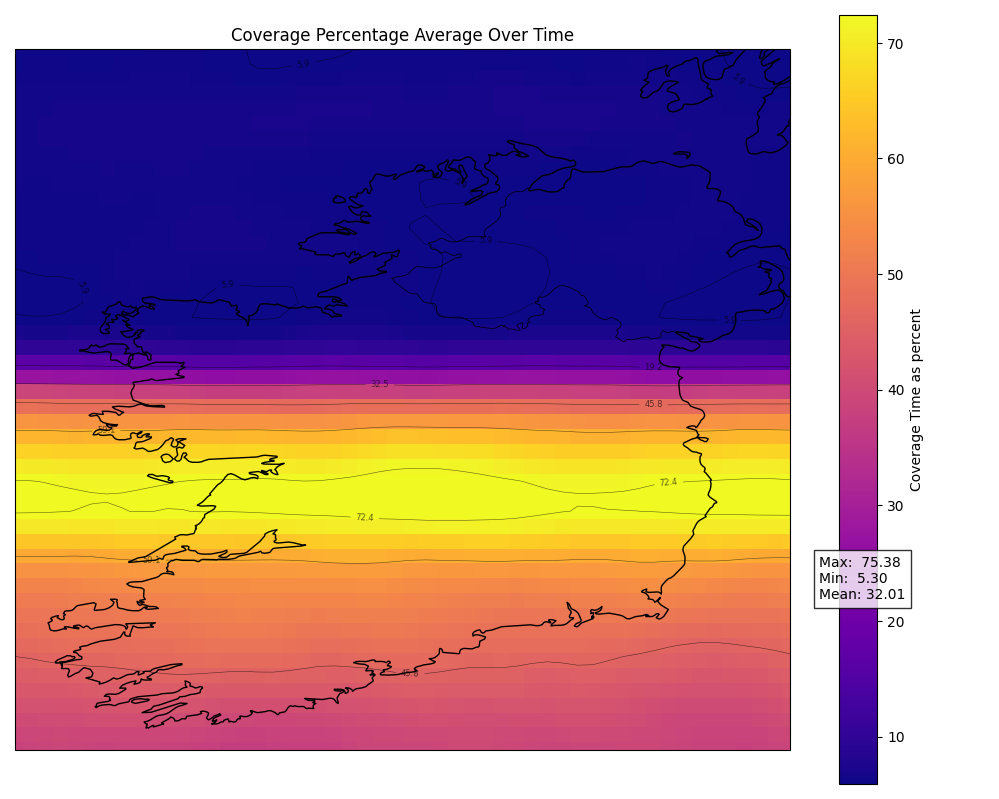
\includegraphics[width=\textwidth]{figures/Coverage_heatmaps/Starlink_all_8am-8pm_coverage_percentage.pdf}
    \caption{Coverage availability as a percentage of time for Starlink over Ireland}
    \label{fig:StarlinkCoverage-percentage}
\end{figure}


Figure \ref{fig:StarlinkCoverage-mbps} shows the average data rate as per the Shannon Capacity formula. With a mean value of 320.33 Mbps and some areas reaching 320.9 Mbps. This is a strong indication that these satellites are capable of 5g speeds. Going off the peal coverage of $375.38\%$ at a peak data rate of $321.30Mbps$, it is possible to expect a peak data rate when coverage is available of $425.84Mbps$.


(THIS FIGURE NEEDS TO BE REGENERATED)
\begin{figure}[h!]
    \centering
    \includegraphics[width=\textwidth]{figures/Coverage_heatmaps/Starlink_all_8am-8pm_mbps.pdf}
    \caption{Average downlink capacity for Starlink over Ireland}
    \label{fig:StarlinkCoverage-mbps}
\end{figure}




\FloatBarrier
\section{OneWeb Simulation - 08:00 to 20:00, 23 April 2026}
\begin{figure}[h!]
    \centering
    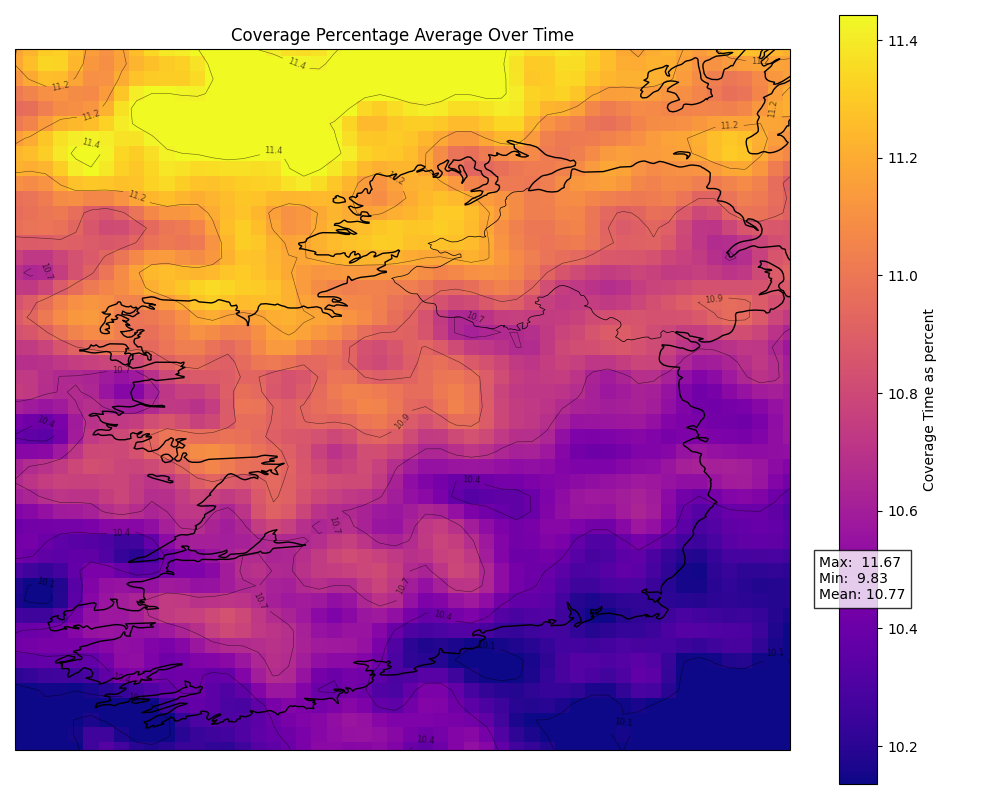
\includegraphics[width=\textwidth]{figures/Coverage_heatmaps/OneWeb_8am-8pm_coverage_percentage.pdf}
    \caption{Coverage availability as a percentage of time for OneWeb over Ireland}
    \label{fig:OneWebCoverage_percentage}
\end{figure}


\begin{figure}[h!]
    \centering
    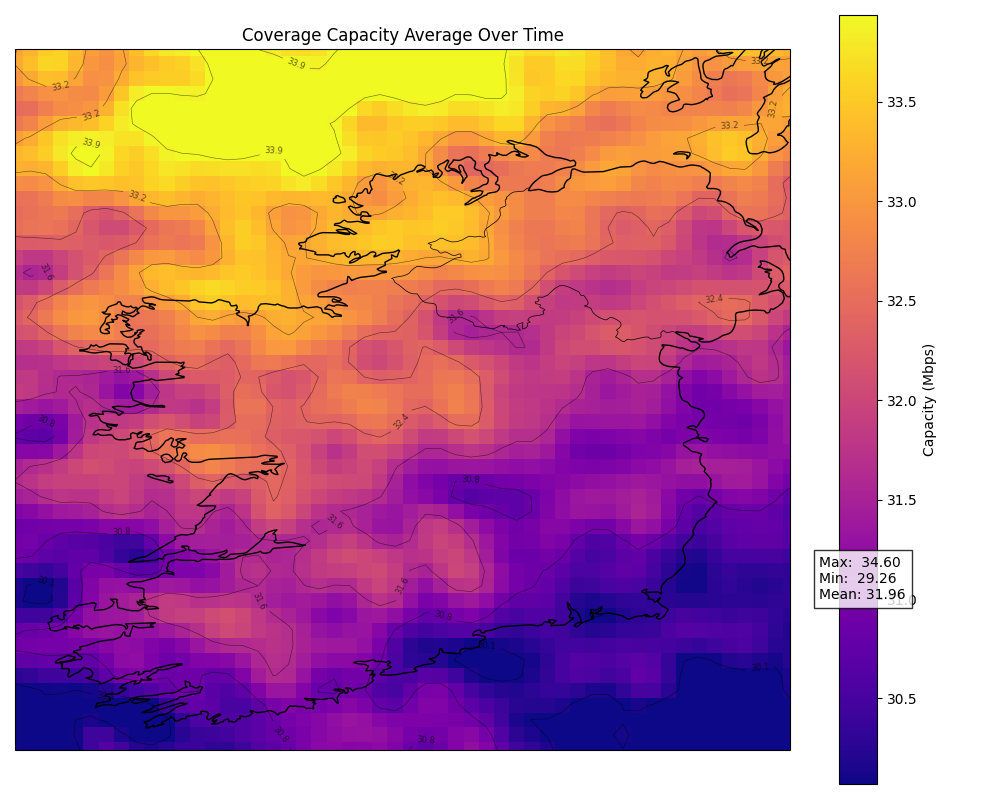
\includegraphics[width=\textwidth]{figures/Coverage_heatmaps/OneWeb_8am-8pm_mbps.pdf}
    \caption{Average downlink capacity for OneWeb over Ireland}
    \label{fig:OneWebCoverage_mbps}
\end{figure}


\FloatBarrier
\section{Kuiper Simulation - 08:00 to 20:00, 23 April 2026}
\begin{figure}[h!]
    \centering
    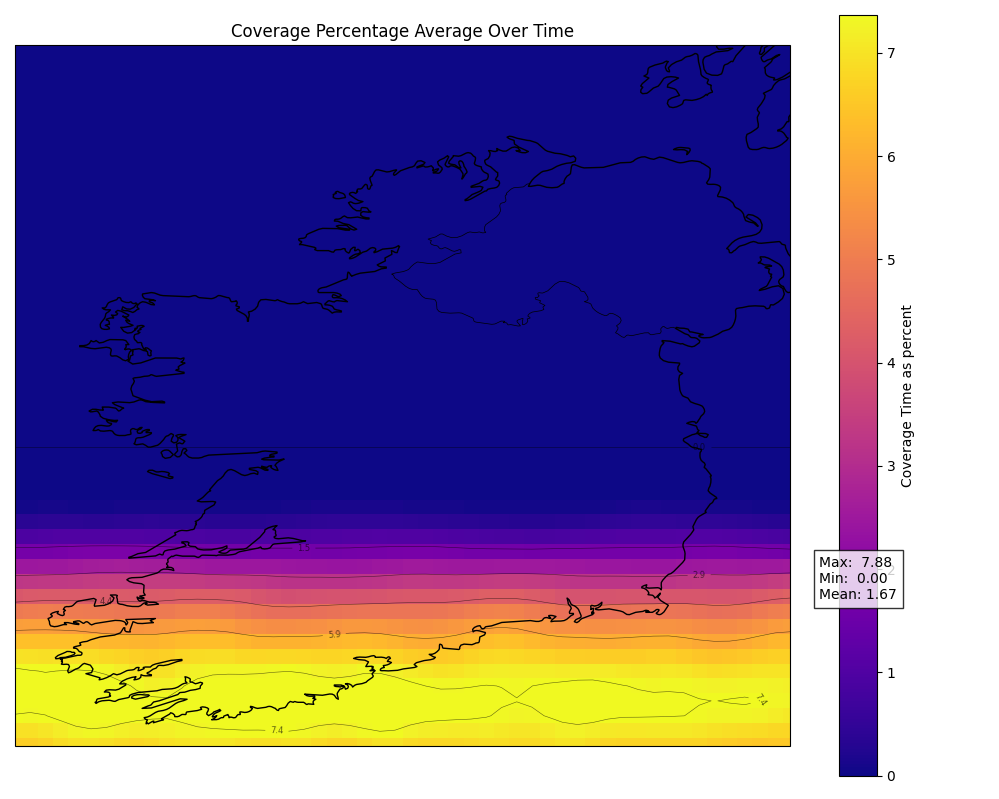
\includegraphics[width=\linewidth]{figures/Coverage_heatmaps/Kuiper_8am-8pm_coverage_percentage.pdf}
    \caption{Coverage availability as a percentage of time for Kuiper over Ireland}
    \label{fig:KuiperCoverage_percentage}
\end{figure}


\begin{figure}[h!]
    \centering
    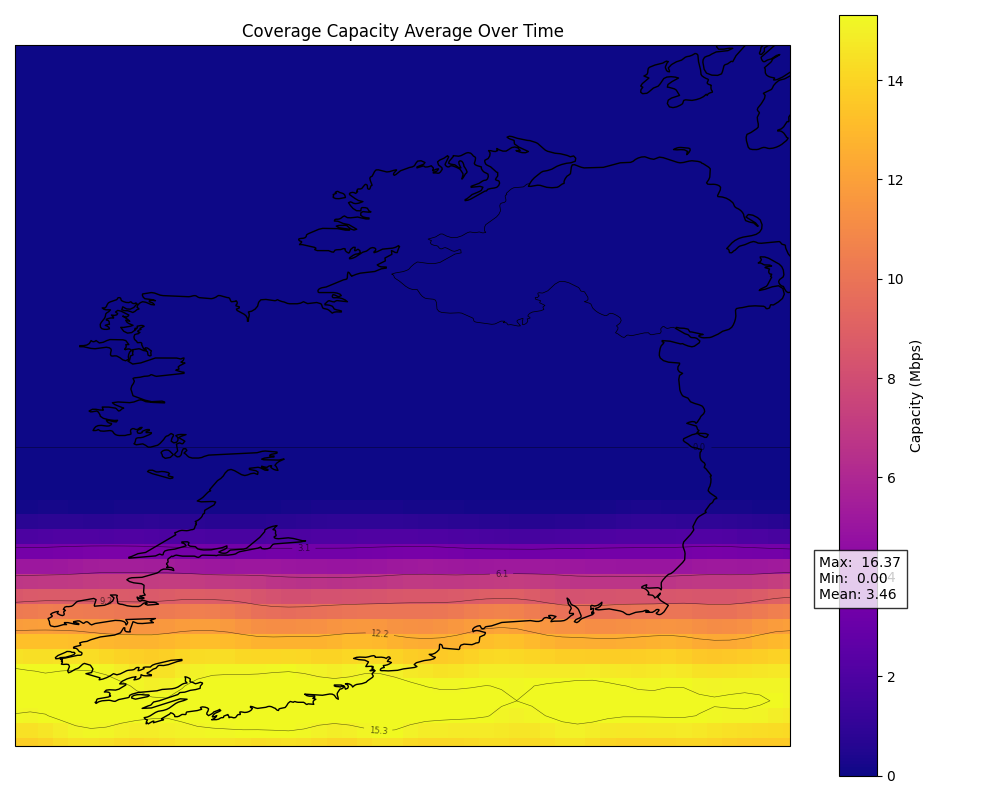
\includegraphics[width=\linewidth]{figures/Coverage_heatmaps/Kuiper_8am-8pm_coverage_mbps.pdf}
    \caption{Average downlink capacity for Kuiper over Ireland}
    \label{fig:KuiperCoverage_mbps}
\end{figure}



\FloatBarrier
\section{Traditional 5G Coverage in Ireland}


\begin{figure}[!ht]
  \centering
  % Row 1
  \begin{subfigure}{0.48\textwidth}
    \centering
    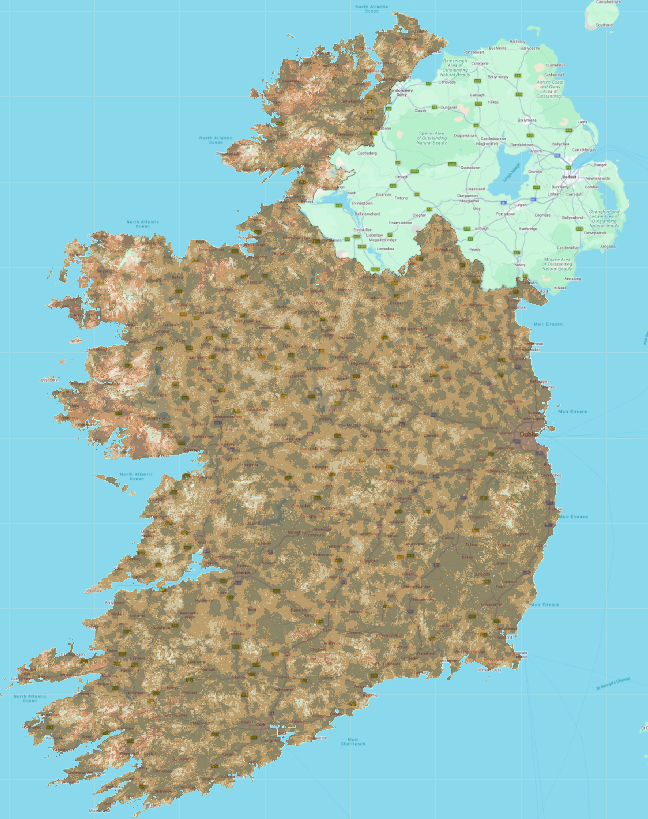
\includegraphics[width=\linewidth]{figures/5g-48.png}
    \caption{5G coverage in Ireland — 48}
  \end{subfigure}
  \hfill
  \begin{subfigure}{0.48\textwidth}
    \centering
    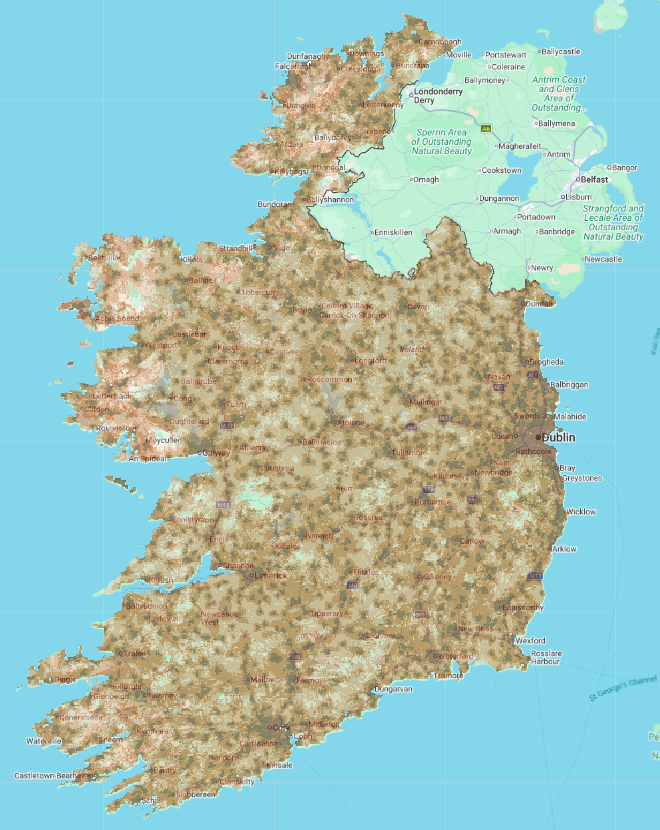
\includegraphics[width=\linewidth]{figures/5g-Eir.png}
    \caption{5G coverage in Ireland — Eir}
  \end{subfigure}

  \bigskip

  % Row 2
  \begin{subfigure}{0.48\textwidth}
    \centering
    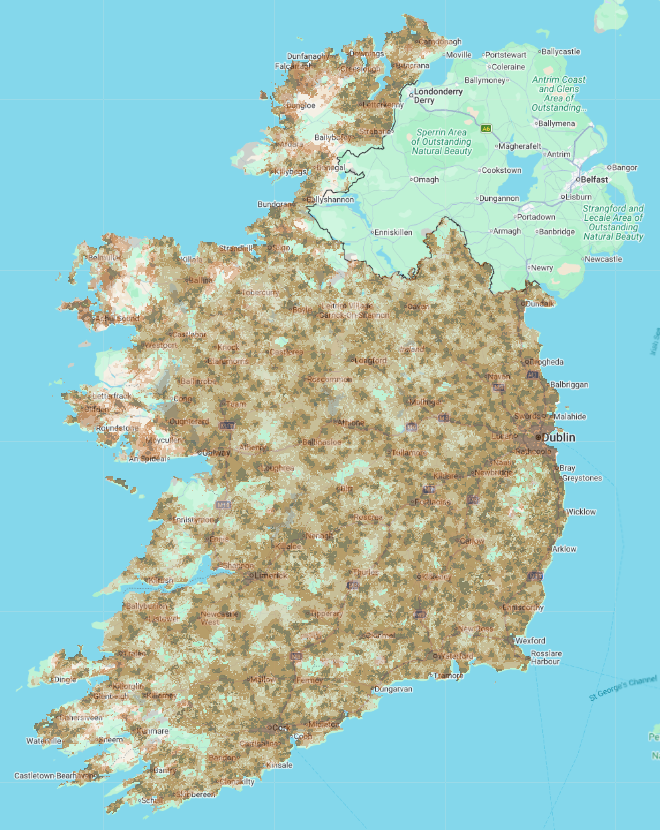
\includegraphics[width=\linewidth]{figures/5g-three.png}
    \caption{5G coverage in Ireland — Three}
  \end{subfigure}
  \hfill
  \begin{subfigure}{0.48\textwidth}
    \centering
    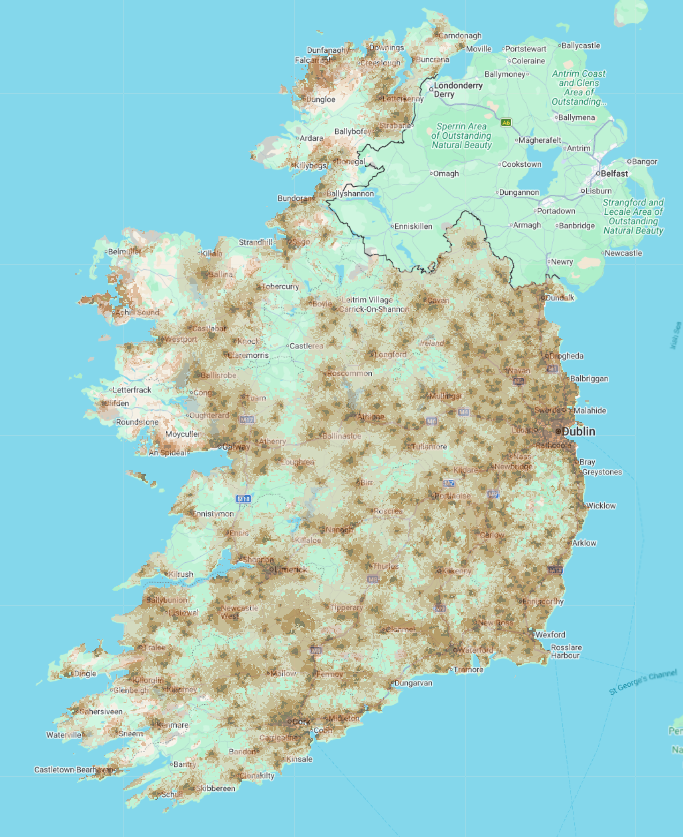
\includegraphics[width=\linewidth]{figures/5g-vodafone.png}
    \caption{5G coverage in Ireland — Vodafone }
  \end{subfigure}

  
\caption{5G coverage in Ireland for different mobile network providers%
\protect\cite{comreg_coverage_map}}

  \label{fig:5g_coverage}
\end{figure}


